\documentclass[acmtog]{acmart}
\usepackage{graphicx}
\usepackage{subfigure}
% Title portion
\title{Assignment 4 : Global illumination using path tracing
\author{Name:\quad Longtian Qiu  \\ student number: \quad 2018533107
	\\email:\quad qiult@shanghaitech.edu.cn }

% Document starts
\begin{document}
\maketitle

\vspace*{2 ex}


\section{Introduction}

In this assignment, a image is generated at ray-based, which means the image is draw one pixel by another.To achieve path-tracing rendering, I generate multiple rays from camera to the scene. Then the ray will bounce among the objects inside the scene and it’s path is decided by BRDF. The result of ray’s every intersection with object is weighted and sum up to the final result of the pixel.
\section{Implementation Details}

Inside <light.hpp> I implement two function. One is to generate a random position inside the area light by random function.Another is to check if the given ray intersect with the light area and is not blocked by other objects inside the scene except for the walls.
Inside <material.hpp> I implement ideal diffuse BRDF and ideal specular BRDF.For eval function of both part, I return the value of the BRDF by the output direction and the norm of the intersecting point. Then for sample function in diffuse, I random choose a point from the sphere with radius 1 and origin at the intersection point. Then the next ray’s direction is from the origin to the selected point.For sample in specular BRDF, the ray’s direction is the reflection of input direction relating to the intersection’s norm direction.
Inside <pathTracingIntegrator.hpp> I implement the rendering based on path tracing. First I generate multiple rays from camera to scene for each pixels and take the average value of the rays at one pixel as the its final color. For each ray, after it reach the first intersection point, the path afterward is decided by the BRDF until it bounces more than the max bounce time or it intersects with nothing. Every time the ray intersect with an object, we add the weighted surface color to the final result and generate multiple rays to the light area to check if the point is affected by the light. If the answer is yes, we add the surface color multiply the cosine of the point’s normal and light direction. Otherwise do nothing.
For the weighted surface color mentioned above, the weight is decided by the probability of the chosen path.
The area light is drawn by checking the distance of the intersection point with the light center. If the distance is less than a certain value, we paint it the light color.
\section{Results}

\begin{figure}[h]
\centering
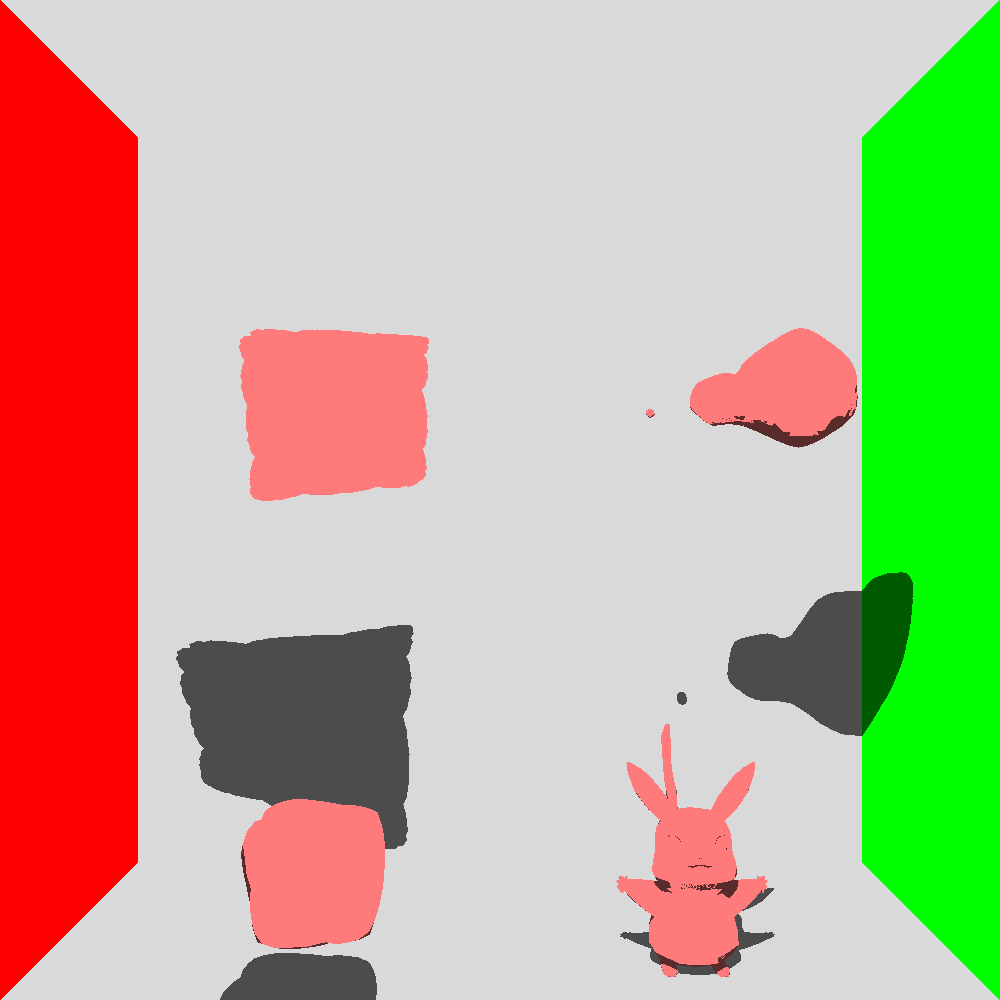
\includegraphics[width=4cm,height=5cm]{output.png}
\caption{With loop subdivision}
\end{figure}



\end{document}
